\chapter{Results and Analyses} \label{chap:result}

This chapter is dedicated not only to give an overview of the results of the simulation, but also to analyse the given results within certain parameters. This chapter is, in essence, where the problem statement in section \vref{sec: Problem Statement} can finally be answered.

The results shown and analysed are all based on the same seed (the seed being 808420), making it possible to reproduce the results both with and without contact tracing. 

We have created our results by simulating 1,000 drops with and without contact tracing enabled. In the following sections the two simulations will be compared, to each other and also to the real world. This is done by plotting the data found in Appendix \ref{Appendix:Data} onto graphs, these then visualises the differences and can be analysed. 

\section{Results from the Simulation}

To create a baseline for the remainder of the results of the simulation results, we will first outline and analyse results from the simulation, with the standard parameters for the virus and contact tracing, which we have defined and described in the previous chapter in section \ref{subsec:Data in Sim}.

\begin{figure}[H]
    \centering
    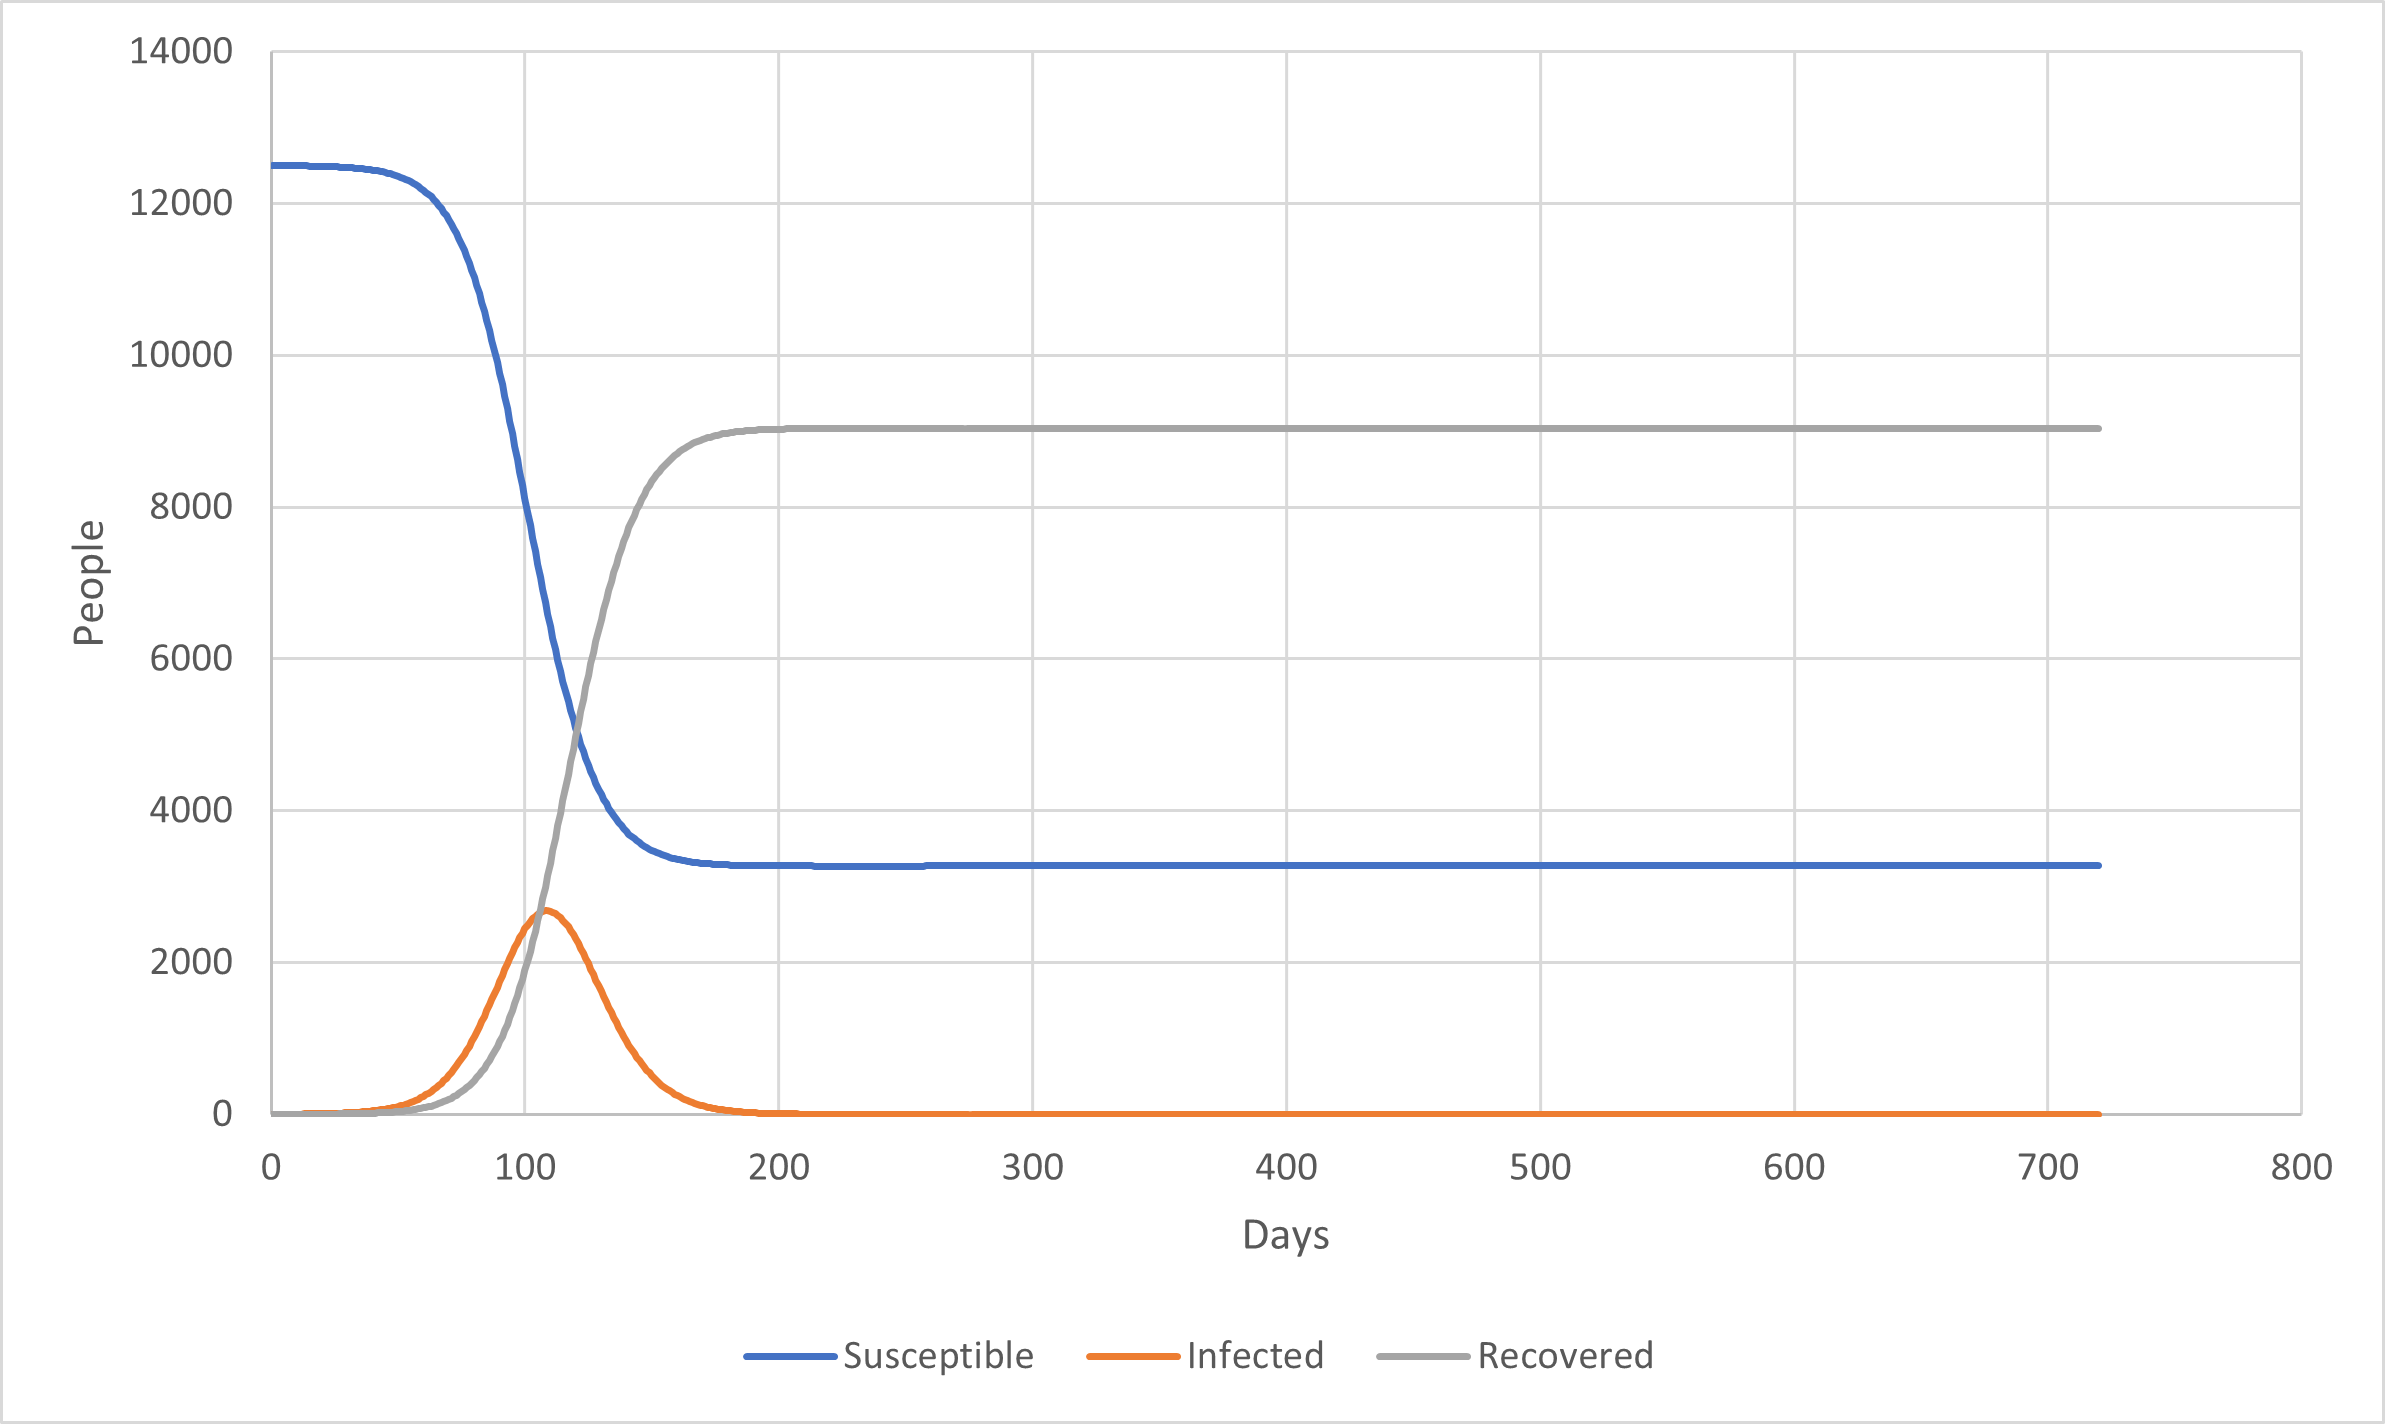
\includegraphics[width=0.75\textwidth]{0_billeder/Sim_CT_OFF.png}
    \caption{Graph of susceptible, infected and recovered plotted against days, from simulation without contact tracing}
    \label{fig:Sim_CT_OFF-1}
\end{figure}

Figure \ref{fig:Sim_CT_OFF-1} is a graph showing how individuals in the population slowly change status throughout the time frame with no contact tracing to mitigate the spread.

As is shown in \ref{fig:Sim_CT_OFF-1}, the infection peaks and dies out rather quickly (within the first 200 days). By the end of the time frame, some people remain uninfected (susceptible), while the majority of the population have recovered. It should be noted that the \say{recovered} state includes those who have survived and succumbed to the infection. This is quite different from figure \ref{fig:Sim_CT_ON-1}, as shown below.

\begin{figure}[H]
    \centering
    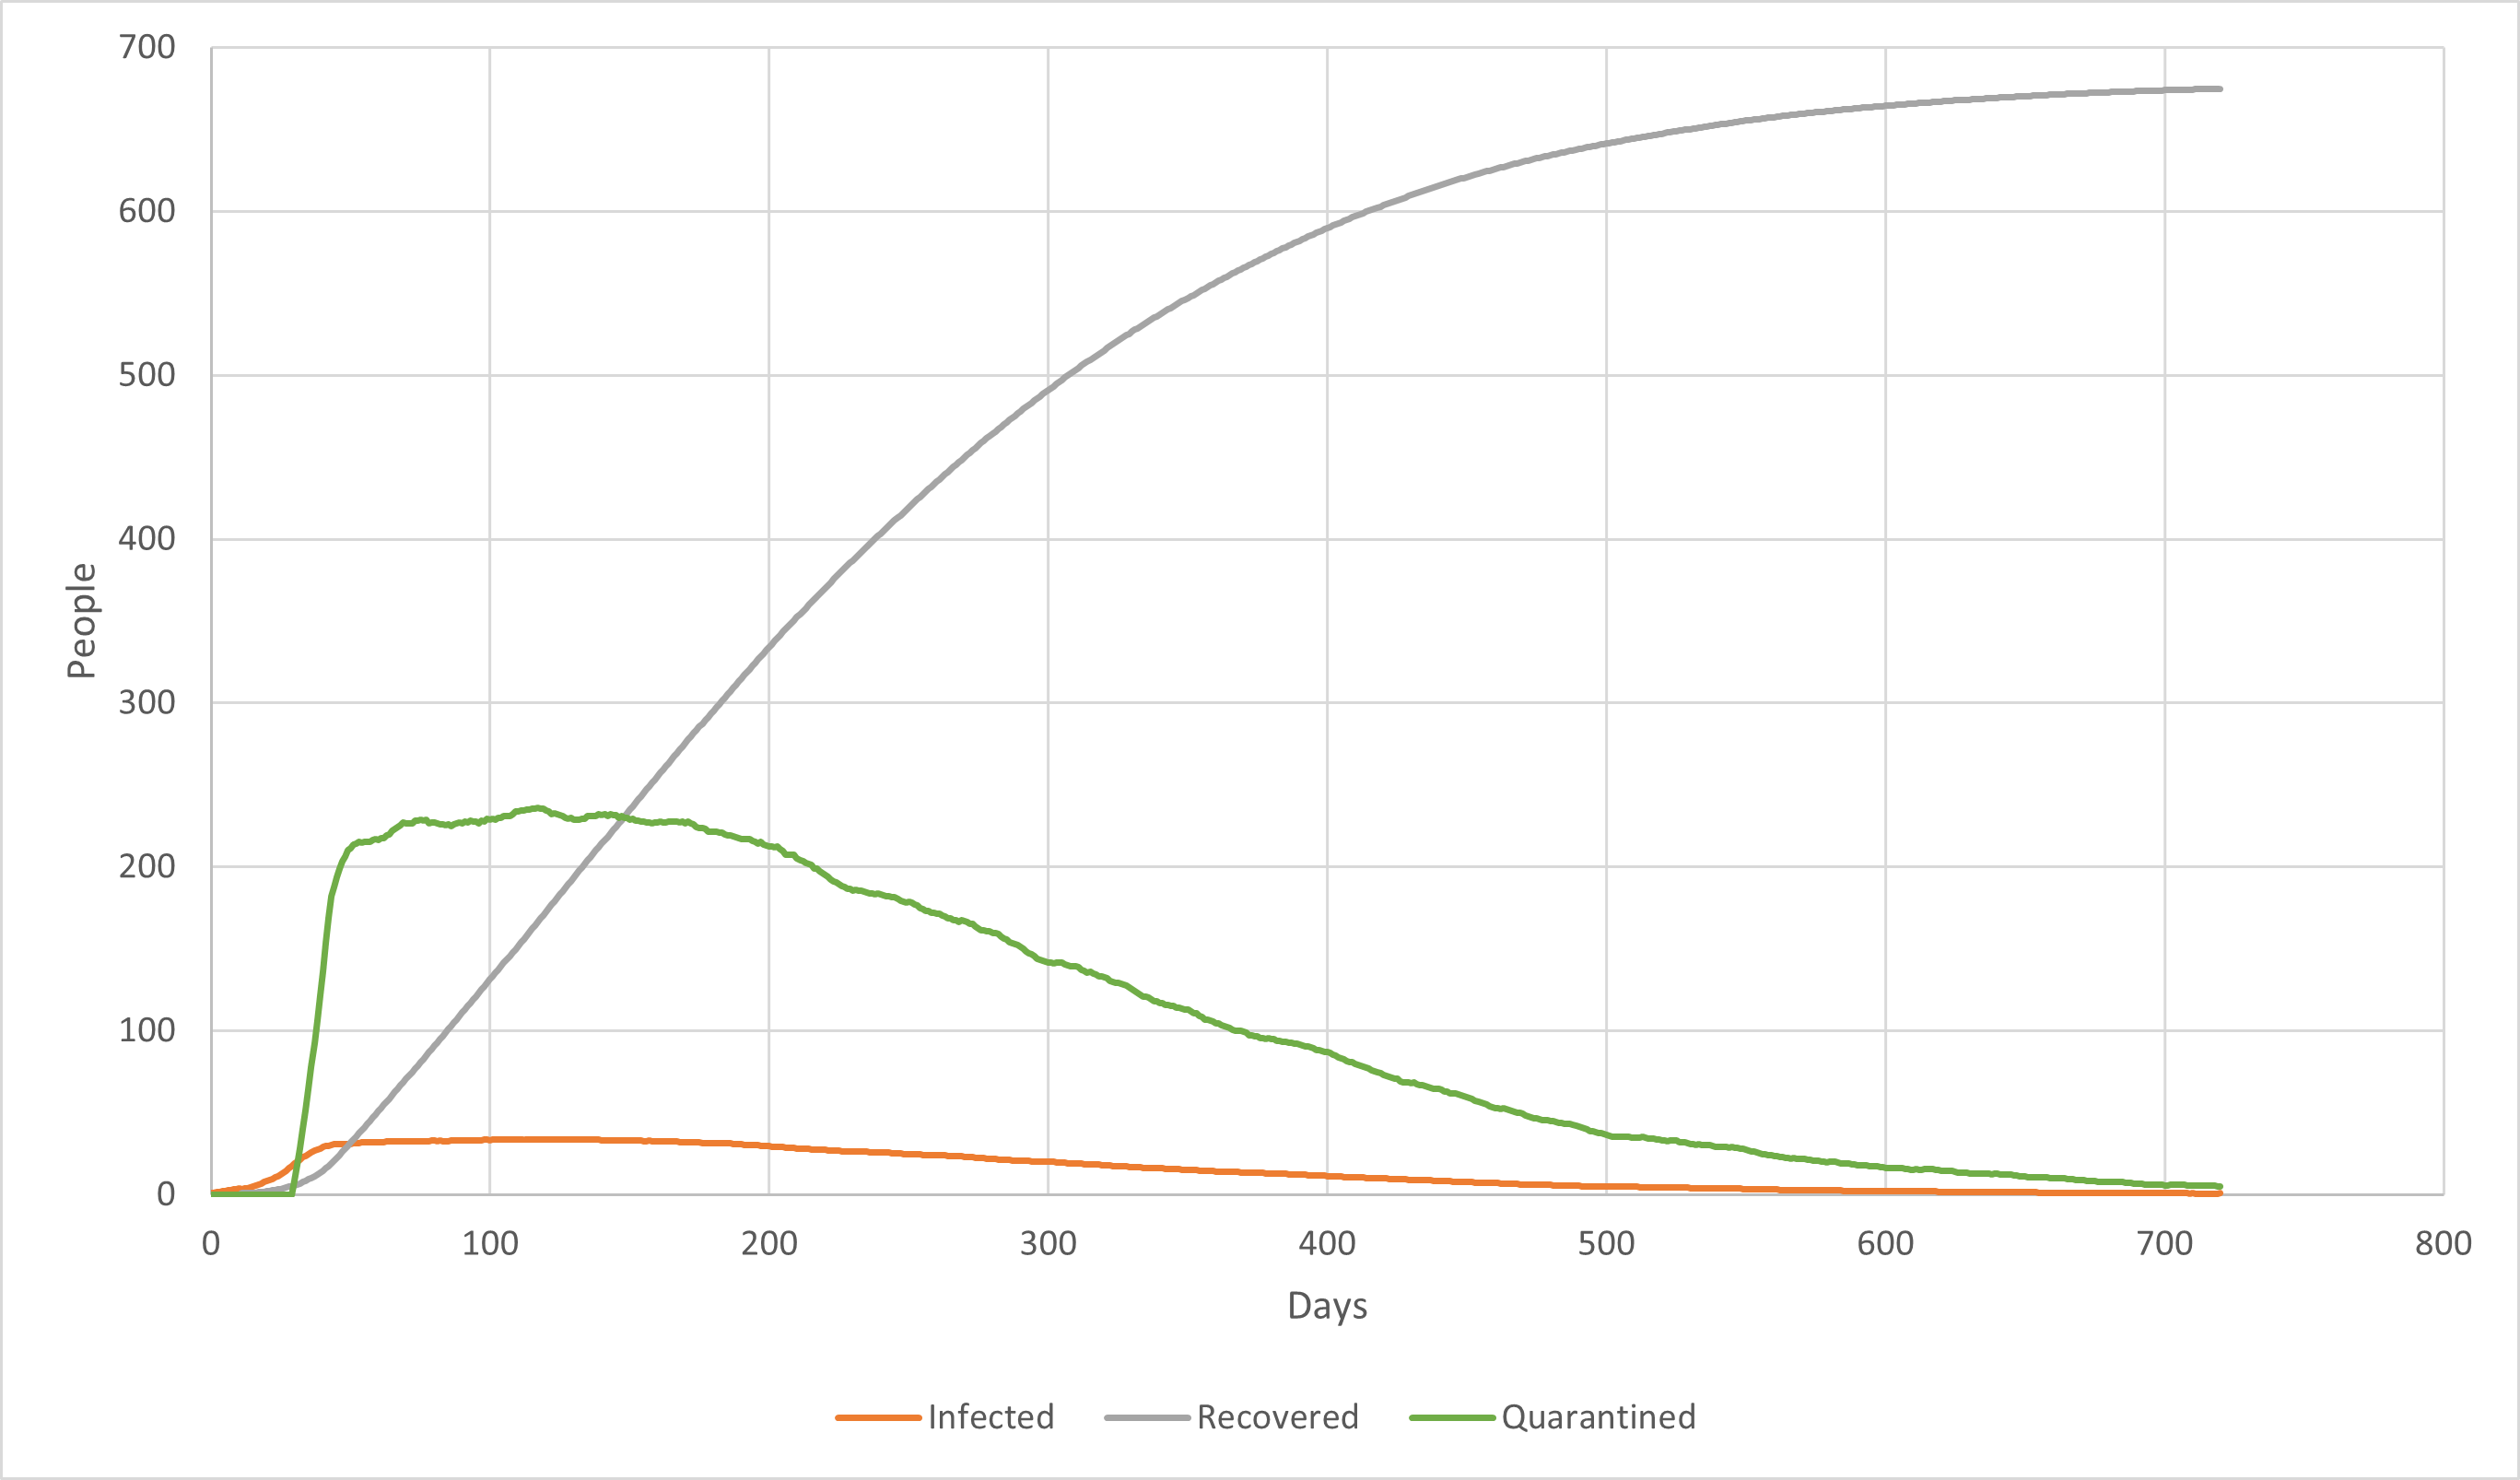
\includegraphics[width=0.75\textwidth]{0_billeder/Sim_CT_ON.png}
    \caption{Graph of quarantined, infected and recovered plotted against days, from simulation with contact tracing}
    \label{fig:Sim_CT_ON-1}
\end{figure}

In figure \ref{fig:Sim_CT_ON-1}, contact tracing has been enabled alongside quarantine. As is shown, this lengthens the infection period for the population as a whole, but greatly diminishes the number of infections across the population. 

Whereas there are about 900 recovered in the simulation run with no contact tracing (figure \ref{fig:Sim_CT_OFF-1}), there are under 700 recovered in the simulation run with contact tracing (figure \ref{fig:Sim_CT_ON-1}). This shows that contact tracing not only lowers the risk of infection to the individual person but also indicates a decrease in deaths (as these are grouped with recovered in the basic simulation).